\section{Partial Optimality for Cubic Clique Partition Problem}
\frame{\tableofcontents[currentsection]}


\begin{frame}
    \frametitle{Partial Optimality for Cubic Clique Partition Problem}
    % mention triple, pairs and constant!!! because we will solve subproblems
    % fix labels if something holds
    % improving map
    % reformulate the problem
    % 2 correct join conditions cannot be combined in the optimal solution
    % so when applied simultaneously they result into a suboptimal solution. 
    % Last: if for every labeling, an improving map fixes the label
    % then we can fix the label and still obtain an optimal solution
    \onslide<1->{
        Extended cost function
        $\cost \colon \binom{\fSet}{3} \cup \binom{\fSet}{2} \cup {\emptyset} \to \real$\\
    }
    \onslide<2->{
        Instance of the extended cubic clique partition problem:
        \[
            \text{\textcolor{red}{
            $\min\limits_{\labels \colon \binom{\fSet}{2} \to \bSet}$
            }}
            \text{\textcolor{blue}{$
            \sum\limits_{abc \in \binom{\fSet}{3}}
            \cost_{abc}\labels_{ab}\labels_{bc}\labels_{ac} 
            + \sum\limits_{ab \in \binom{\fSet}{2}}
            \cost_{ab}\labels_{ab}
            + \cost_{\emptyset}
            $}
            }
        \]\\
        subject to 
        $\labels_{ab} + \labels_{bc} - 1 \leq \labels_{ac}$
        for all distinct $a,b,c \in \fSet$.\\
    }
    \vspace{10px}
    \onslide<3->{
        Let $\allL \neq \emptyset$, 
        $\obj \colon \allL \to \real$ and
        $\impmap \colon \allL \to \allL$. 
        $\impmap$ is an \textbf{Improving Map} for 
        for the problem 
        $\min\limits_{\labels \in \allL}\obj$
        if for every $\labels \in \allL$:
        $\obj(\impmap(\labels)) \leq \obj(\labels)$.\\
    }
    \vspace{5px}
    \onslide<4->{
        Moreover, let $Q \subseteq Y$
        and $\impmap$ an improving map.
        If for every $\labels \in \allL$,
        $\impmap(\labels) \in Q$,
        then there is an optimal solution  $\labels^* \in Q$.
        to $\min\limits_{\labels \in \allL}\obj$.
    }
    \vspace{5px}
    \onslide<5->{
        Let 
        $\allL \subseteq \{\text{feasible }y \mid \labels \colon \binom{\fSet}{2} \to \bSet\}$,
        $\text{\textcolor{blue}{$\obj_{\cost}$}} \colon \allL \to \real$
        and $\impmap$ an improving map.
        If for every $\labels \in \allL$:
        $\impmap(\labels)_{ab} = \beta$,
        $ab \in \binom{\fSet}{2}$, $\beta \in \bSet$, 
        then there is an optimal solution $\labels^*$
        to $\text{\textcolor{red}{$\min\limits_{\labels \in \allL}$} \textcolor{blue}{$\obj_{\cost}$}}$
        such that $\labels^*_{ab} = \beta$.
    }
\end{frame}

\begin{frame}
    \frametitle{Pair-CUT Partial Optimality Condition}
    % partial optimality conditions by constructing improving maps
    % to fix some labels if certain conditions hold
    % cut samples $i,j$ if
    % the direct joing penalty $\geq$
    % the sum of rewards for joining
    % some subset $\subR$ with $i \in \subR$ 
    % and $\overline{\subR}$ with $j \in \overline{\subR}$
    % ($\approx$ i-j min-cut)\\
    Let $ij \in \binom{\fSet}{2}$.
    If there exists $\subR \subseteq \fSet$
    such that $i \in \subR \land j \notin \subR$ and
    \[
        \cost^+_{ij} \geq 
        \sum\limits_{p \in \subR \land q,r \notin \subR \;\lor\; p,q \in \subR \land r \notin \subR}
        \cost^-_{pqr} +
        \sum\limits_{p \in \subR \land q \notin \subR}
        \cost^-_{pq}
    \]
    then there is an optimal solution $\labels^*$
    to $\text{\textcolor{red}{$\min\limits_{\labels \in \allL}$} \textcolor{blue}{$\obj_{\cost}$}}$
    such that $\labels^*_{ij} = 0$.\\
    \vspace{10px}

    \onslide<2->{
    \begin{minipage}{0.48\textwidth}
        \centering
        Cut a and b?\\
        \begin{tikzpicture}[node distance=30px]
            % nodes
            \node[state] (a) {a};
            \node[state] (b) [right of=a] {b};
            \node[state] (c) [below of=a] {c};
            \node[state] (d) [right of=b] {d};
            \node[state] (e) [below of=b] {e};
            % edges
            \path[-] (a) edge node[left] {\footnotesize -10} (c);
            \path[-] (a) edge node[above] {\footnotesize 5} (b);
            \path[-] (a) edge node[] {\footnotesize } (e);
            \path[-] (c) edge node[below] {\footnotesize -1} (e);
            \path[-] (b) edge node[above left=1px] {\footnotesize -3} (e);
            \path[-] (b) edge node[below left] {\footnotesize -3} (d);
            \path[-] (e) edge node[] {\footnotesize } (d);
        \end{tikzpicture}
    \end{minipage}  
    }
    \onslide<3->{
    \begin{minipage}{0.48\textwidth}
        \centering
        a-b Min-Cut\\
        \begin{tikzpicture}[node distance=30px]
            % nodes
            \node[state, draw=red] (a) {a};
            \node[state, draw=blue] (b) [right of=a] {b};
            \node[state, draw=red] (c) [below of=a] {c};
            \node[state, draw=blue] (d) [right of=b] {d};
            \node[state, draw=blue] (e) [below of=b] {e};
            % edges
            \path[-] (a) edge[red] node[left] {\footnotesize -10} (c);
            \path[-] (a) edge node[above] {\footnotesize 5} (b);
            \path[-] (a) edge[above right] node[] {\footnotesize -3} (e);
            \path[-] (c) edge node[below] {\footnotesize -1} (e);
            \path[-] (b) edge[blue] node[] {\footnotesize} (e);
            \path[-] (b) edge[blue] node[below left] {\footnotesize -3} (d);
            \path[-] (e) edge[blue] node[] {\footnotesize } (d);
        \end{tikzpicture}
    \end{minipage}\\
    }
    \vspace{5px}
    \onslide<4->{
    Improving map $\impmap: \allL \to \allL$
    for $\labels \in \allL$ and $pq \in \binom{\fSet}{2}$:
    \[
        \begin{cases}
            \impmap(\labels)_{pq} = 0 & \labels_{ij}=1 \land |\{p,q\} \cap \subR| = 1\\
            \impmap(\labels)_{pq}=\labels_{pq} & otherwise
        \end{cases}
    \]
    }
\end{frame}


\begin{frame}
    \frametitle{Partial Optimality Conditions}
    \textbf{Partial Optimality Conditions:}
    \begin{enumerate}
        \item Subproblem-CUT-condition (cut subset from its complement)
        \item CUT-conditions (cut pairs and triples)
        \item JOIN-conditions (join subsets, pairs and triples)
    \end{enumerate}
    \vspace{10px}
    \onslide<2->{
    CUT-conditions can be applied simultaneously.\\
    \vspace{5px}
    JOIN-conditions must be applied iteratively!\\
    \vspace{5px}
    $Q_1, Q_2 \in \allL$:
    if there exists an optimal $\labels^*_1 \in Q_1$ and
    there exists an optimal $\labels^*_2 \in Q_2$ 
    $\nrightarrow$ there is an optimal $\labels^* \in Q_1 \cap Q_2$:\\
    \vspace{5px}
    \begin{minipage}{0.78\textwidth}
        $\min\limits_{\labels \in \allL}\obj_{\cost} = -2$\\
        $Q_1 = \{\labels \in \allL \mid \labels_{ab} = 1\}$\\
        $Q_2 = \{\labels \in \allL \mid \labels_{ac} = 1\}$\\
        $\to Q_1 \cap Q_2 = \{\labels \in \allL \mid \labels_{ab} = 1 \land \labels_{ac} = 1\}$
        $\lightning$
    \end{minipage}
    \begin{minipage}{0.2\textwidth}
        \centering
        \begin{tikzpicture}[node distance=30px]
                % nodes
                \node[state] (a) {a};
                \node[state] (b) [above right of=a] {b};
                \node[state] (c) [below right of=b] {c};
                % edges
                \path[-] (a) edge[] node[left] {\footnotesize -2} (b);
                \path[-] (b) edge[] node[right] {\footnotesize -2} (c);
                \path[-] (c) edge[] node[below] {\footnotesize -2} (a);
                \path[-] (a) edge[] node[above=3px] {\footnotesize 5} (c);    
        \end{tikzpicture}
    \end{minipage}\\
    }
    \vspace{5px}
    \onslide<3->{
    Apply partial optimality conditions $\to$ solve subproblems!
    }
\end{frame}


\begin{frame}
    \frametitle{Partial Optimality Algorithm}
    \onslide<1->{
    \textbf{Partial Optimality Algorithm:\\}
    \hspace{10px}\textbf{Input:} labeling $\labels$ without fixed labels
    \begin{algorithmic}
        \While{condition applied}
            \State apply subproblem-CUT-condition exhaustively
            \State apply one of JOIN-conditions (in effective order)
        \EndWhile
        \State apply CUT-conditions exhaustively
    \end{algorithmic}
    \hspace{10px}\textbf{Output:} partially optimal labeling $\labels$ with some fixed labels
    }
    \vspace{10px}
    \onslide<2->{
    \textbf{Reduction to subproblems:}
    \begin{enumerate}
        \item Subproblem-CUT-condition:
        fix 0-labels for element pairs from different sample subsets; 
        solve each subset as an independent problem;
        accumulate the results in $\cost_{\emptyset}$;
        \onslide<3->{
        \item JOIN-Conditions: 
        fix 1-labels for elements of the sample subset; 
        add the join-cost to $\cost_{\emptyset}$;
        solve the problem where the subset is considered as one sample;
        }
    \end{enumerate}
    }
\end{frame}


\begin{frame}
    \frametitle{Subproblem-CUT and Subset-JOIN}
    % A couple of words about the split and the implementation
    % apply exhaustively
    % intuition 3.1 and 3.11!!!
    % 3.11 adjustment (abc skipped, acd + b would be skipped!)
    \onslide<1->{
    \textbf{Subproblem-CUT:} cut sample subsets $\subR_1, \subR_2, \dots, \subR_k$
    that are only connected via non-negative costs (applied if $k > 1$)\\
    }
    \vspace{5px}
    \onslide<2->{
    \textbf{Subset-JOIN:} join sample subset $\subR$ with only non-positive costs
    if its worst bipartition joining cost is less than or equal to
    the reward of joining $\subR$ with $\overline{\subR}$ (applied if $|\subR| > 1$)\\
    (the worst bipartition joining cost $\approx$ min-cut)\\
    }
    \vspace{15px}
    \onslide<3->{
        \begin{tikzpicture}[node distance=30px]
            % nodes
            \node[state] (a) {a};
            \node[state] (b) [below left of=a] {b};
            \node[state] (c) [below right of=b] {c};
            \node[state] (d) [above right of=c] {d};
            \node[state] (e) [below right of=d] {e};
            \node[state] (f) [above right of=e] {f};
            \node[state] (h) [below of=e] {h};
            \node[state] (g) [above of=d] {g};
            \node[state] (i) [above of=f] {i};
            % edges
            \path[-] (a) edge node[below right=3px, below] {\footnotesize -1} (b);
            \path[-] (a) edge node {} (c);
            \path[-] (b) edge node {} (c);
            \path[-] (a) edge node[below left=3px, below] {\footnotesize -15} (d);
            \path[-] (c) edge node {} (d);
            \path[-] (d) edge node {} (g);
            \path[-] (d) edge node {} (f);
            \path[-] (g) edge node {} (i);
            \path[-] (i) edge node[above left] {\footnotesize -10} (f);
            \path[-] (g) edge node[below left] {\footnotesize -2} (f);
            \path[-] (d) edge node {} (e);
            \path[-] (e) edge node {} (f);
            \path[-] (e) edge node {} (h);
            \path[-] (d) edge node[right=-3px] {\tiny 50} (h);
            \path[-] (h) edge node[left=-4px] {\tiny -50} (f);
        \end{tikzpicture}
    }
    \hspace{5px}
    \onslide<4->{
        \begin{tikzpicture}[node distance=30px]
            % nodes
            \node[state] (acd) {acd};
            \node[state] (b) [left of=acd] {b};
            \node[state] (e) [below right of=acd] {e};
            \node[state] (f) [above right of=e] {f};
            \node[state] (h) [below of=e] {h};
            \node[state] (g) [above of=acd] {g};
            \node[state] (i) [above of=f] {i};
            % edges
            \path[-] (acd) edge node[above] {\footnotesize -1} (b);
            \path[-] (acd) edge node {} (g);
            \path[-] (acd) edge node {} (f);
            \path[-] (g) edge node {} (i);
            \path[-] (i) edge node[above left] {\footnotesize -10} (f);
            \path[-] (g) edge node[below left] {\footnotesize -2} (f);
            \path[-] (acd) edge node {} (e);
            \path[-] (e) edge node {} (f);
            \path[-] (e) edge node {} (h);
            \path[-] (acd) edge node[right=-3px] {\tiny 50} (h);
            \path[-] (h) edge node[left=-4px] {\tiny -50} (f);
        \end{tikzpicture}
    }
    \onslide<5->{
        \begin{tikzpicture}[node distance=30px]
            % nodes
            \node[state] (acd) {acd};
            \node[state] (b) [above of=acd] {b};
            \node[state] (efghi) [below of=acd] {efghi};
            % edges
            \path[-] (acd) edge node[right] {\footnotesize -1} (b);
            \path[-] (acd) edge node[right] {\footnotesize 48} (efghi);
        \end{tikzpicture}
    }
    \onslide<6->{
        \begin{tikzpicture}[node distance=30px]
            % nodes
            \node[state] (acd) {acd};
            \node[state] (b) [above of=acd] {b};
            \node[state] (efghi) [below of=acd] {efghi};
            % edges
            \path[-] (acd) edge node[right] {\footnotesize -1} (b);
        \end{tikzpicture}
    }
    \onslide<7->{
        \begin{tikzpicture}[node distance=30px]
            % nodes
            \node[state] (abcd) {abcd};
            \node[state] (efghi) [below of=acd] {efghi};
        \end{tikzpicture}
    }
    \\
    \hspace{20px}
    \onslide<3->{$\cost_{\emptyset}=0$}
    \hspace{60px}
    \onslide<4->{$\cost_{\emptyset}=-15$}
    \hspace{25px}
    \onslide<5->{$\cost_{\emptyset}=-75$}
    \hspace{15px}
    \onslide<7->{$\cost_{\emptyset}=-76$}
\end{frame}


\begin{frame}
    \frametitle{Other JOIN-conditions}
    \onslide<1->{
        \textbf{Pair-JOIN-1:} join samples $ij \in \binom{\fSet}{2}$ if
        their overall joining reward $\geq$
        the sum of rewards and penalties for joining
        some subset $\subR$ with $i \in \subR \land j \notin \subR$ 
        with $\overline{\subR}$
        ($\approx$ i-j min-cut)\\
    }
    \vspace{10px}
    \onslide<2->{
        \textbf{Pair-JOIN-2:} join samples $ik \in \binom{\fSet}{2}$ if 
        there exist $ijk \in \binom{\fSet}{3}$ that fulfills 
        3 conditions
        ($\approx$ i-jk min-cut, $\approx$ ij-k min-cut, 1 explicit condition)\\
    }
    \vspace{10px}
    \onslide<3->{
        \textbf{Pair-JOIN-3:} join samples $ij \in \binom{\fSet}{2}$ if
        $\cost_{ij}\leq$ 
        the sum of reward costs for joining pairs and triples 
        containing $i$ or $j$\\
    }
    \vspace{10px}
    \onslide<4->{
        \textbf{Pair-JOIN-4:} join samples $ik \in \binom{\fSet}{2}$
        if there exists $ijk \in \binom{\fSet}{3}$ such that 
        7 explicit conditions hold\\
    }
    \vspace{10px}
    \onslide<5->{
        \textbf{Triple-JOIN:} join samples $ijk \in \binom{\fSet}{3}$ 
        if the condition holds\\ 
        (similar to Pair-JOIN-1)
        ($\approx$ i-jk min-cut)\\
    }
    
\end{frame}


\begin{frame}
    \frametitle{Pyramid Instance and CUT-conditions}
    \vspace{-5px}
    $\cost_{bcd}=10$\\
    $\cost_{abc}=\cost_{abd}=\cost_{acd}=-50$\\
    \vspace{5px}
    \onslide<1->{    
        \begin{tikzpicture}[node distance=30px]
            % nodes
            \node[state] (a) {a};
            \node[state] (b) [below left of=a, below=5px] {b};
            \node[state] (c) [below right of=a, right=10px] {c};
            \node[state] (d) [below right of=b] {d};
            % edges
            \path[-] (a) edge node {} (b);
            \path[-] (a) edge node {} (c);
            \path[-] (a) edge node {} (d);
            \path[-, dashed] (b) edge node {} (c);
            \path[-] (c) edge node {} (d);
            \path[-] (d) edge node {} (b);
        \end{tikzpicture}
    }
    \onslide<2->{ 
        \hspace{20px}   
        \begin{tikzpicture}[node distance=30px]
            % nodes
            \node[state] (ac) {ac};
            \node[state] (b) [below left of=a] {b};
            \node[state] (d) [below right of=a] {d};
            % edges
            \path[-] (ac) edge node[above left=-3px] {\footnotesize-50} (b);
            \path[-] (ac) edge node[above right=-3px] {\footnotesize-50} (d);
            \path[-] (d) edge node[above] {\footnotesize-40} (b);
        \end{tikzpicture}
    }
    \hspace{10px}
    \onslide<3->{ 
        \hspace{30px} 
        \begin{tikzpicture}[node distance=30px]
            % nodes
            \node[state] (abcd) {abcd};
        \end{tikzpicture}   
    }\\
    \hspace{40px}
    \onslide<2->{Pair-JOIN-2}
    \hspace{45px}
    \onslide<3->{
        Subset-JOIN
        \hspace{10px}
        $\cost_{\emptyset}=-140$
    }
    
    \vspace{10px}
    \onslide<4->{
        \textbf{Pair-CUT:} cut samples $i,j$ if
        the direct joing penalty $\geq$
        the sum of rewards for joining
        some subset $\subR$ with $i \in \subR \land j \notin \subR$ 
        with $\overline{\subR}$\\
        ($\approx$ i-j min-cut)\\
    }
    \vspace{5px}
    \onslide<5->{
        \textbf{Triple-CUT:} cut samples $i,j,k$ 
        if the condition holds\\ 
        (similar to Pair-CUT)
        ($\approx$ i-jk min-cut)\\
    }
    \vspace{10px}
    \onslide<6->{
        Samples in the pyramid with $\cost_{bcd}=100$ are unjoinable!\\
        Triple-CUT is applied to the triple $bcd$
    }
\end{frame}


\begin{frame}
    \frametitle{Program Structure}
    % Features: ClusteringProblem is generally defined for all types of Cubic Clique Partition Problem (not necessarily points),
    %     cost function + sparse costs!, label computation, cut triples,
    %     logs joins and cuts!
    \begin{figure}[h]
        \centering
        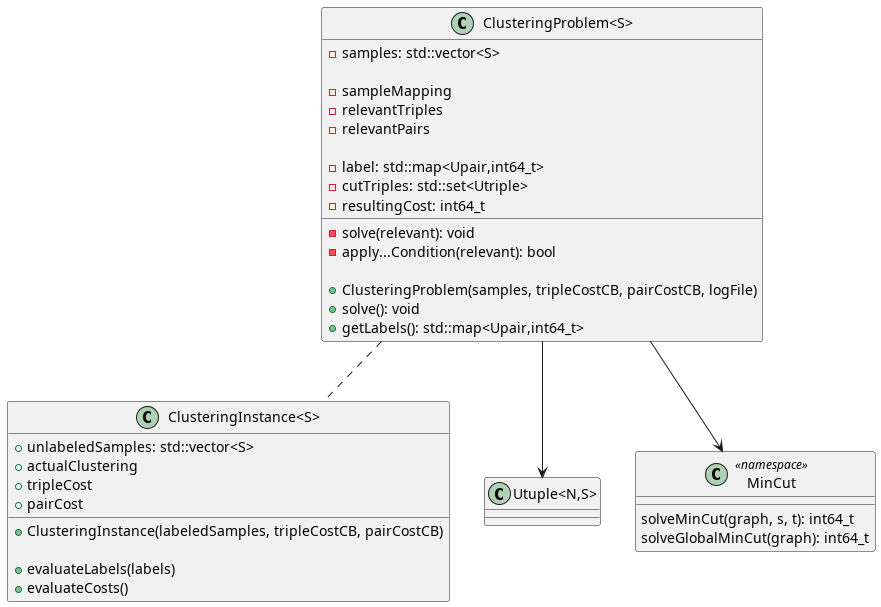
\includegraphics[width=\textwidth]{Program.png}
    \end{figure}
\end{frame}






